\documentclass[supercite]{Experimental_Report}

\title{~~~~~~数据结构实验~~~~~~}
\author{张家豪}
\school{计算机科学与技术学院}
\classnum{CS2104}
\stunum{U202115434}
\instructor{袁凌} % 李平、孙伟平、范晔斌、陈加忠
\date{2021年6月10日}

\usepackage{algorithm, multirow}
\usepackage{algpseudocode}
\usepackage{amsmath}
\usepackage{amsthm}
\usepackage{framed}
\usepackage{mathtools}
\usepackage{subcaption}
\usepackage{xltxtra} %提供了针对XeTeX的改进并且加入了XeTeX的LOGO, 自动调用xunicode宏包(提供Unicode字符宏)
\usepackage{bm}
\usepackage{tikz}
\usepackage{tikzscale}
\usepackage{pgfplots}
\usepackage{listings}
%\usepackage{enumerate}

\lstset{
		columns=fixed,       
		numbers=left,                                        % 在左侧显示行号
		numberstyle=\tiny\color{gray},                       % 设定行号格式
		frame=none,                                          % 不显示背景边框
		backgroundcolor=\color[RGB]{245,245,244},            % 设定背景颜色
		keywordstyle=\color[RGB]{40,40,255},                 % 设定关键字颜色
		numberstyle=\footnotesize\color{darkgray},           
		commentstyle=\it\color[RGB]{0,96,96},                % 设置代码注释的格式
		stringstyle=\rmfamily\slshape\color[RGB]{128,0,0},   % 设置字符串格式
		showstringspaces=false,                              % 不显示字符串中的空格
		language=c++,                                        % 设置语言
	}

\pgfplotsset{compat=1.16}

\newcommand{\cfig}[3]{
  \begin{figure}[htb]
    \centering
    \includegraphics[width=#2\textwidth]{images/#1.tikz}
    \caption{#3}
    \label{fig:#1}
  \end{figure}
}

\newcommand{\sfig}[3]{
  \begin{subfigure}[b]{#2\textwidth}
    \includegraphics[width=\textwidth]{images/#1.tikz}
    \caption{#3}
    \label{fig:#1}
  \end{subfigure}
}

\newcommand{\xfig}[3]{
  \begin{figure}[htb]
    \centering
    #3
    \caption{#2}
    \label{fig:#1}
  \end{figure}
}

\newcommand{\rfig}[1]{\autoref{fig:#1}}
\newcommand{\ralg}[1]{\autoref{alg:#1}}
\newcommand{\rthm}[1]{\autoref{thm:#1}}
\newcommand{\rlem}[1]{\autoref{lem:#1}}
\newcommand{\reqn}[1]{\autoref{eqn:#1}}
\newcommand{\rtbl}[1]{\autoref{tbl:#1}}

\algnewcommand\Null{\textsc{null }}
\algnewcommand\algorithmicinput{\textbf{Input:}}
\algnewcommand\Input{\item[\algorithmicinput]}
\algnewcommand\algorithmicoutput{\textbf{Output:}}
\algnewcommand\Output{\item[\algorithmicoutput]}
\algnewcommand\algorithmicbreak{\textbf{break}}
\algnewcommand\Break{\algorithmicbreak}
\algnewcommand\algorithmiccontinue{\textbf{continue}}
\algnewcommand\Continue{\algorithmiccontinue}
\algnewcommand{\LeftCom}[1]{\State $\triangleright$ #1}

\newtheorem{thm}{定理}[section]
\newtheorem{lem}{引理}[section]

\colorlet{shadecolor}{black!15}

\theoremstyle{definition}
\newtheorem{alg}{算法}[section]

\def\thmautorefname~#1\null{定理~#1~\null}
\def\lemautorefname~#1\null{引理~#1~\null}
\def\algautorefname~#1\null{算法~#1~\null}

\begin{document}

\maketitle

\clearpage

\pagenumbering{Roman}

\tableofcontents[level=3]

\clearpage

\pagenumbering{arabic}

\section{基于顺序存储结构的线性表实现}

\subsection{实验目的}

通过实验达到:

(1)加深对线性表的概念、基本运算的理解;

(2)熟练掌握线性表的逻辑结构与物理结构的关系;

(3)物理结构采用顺序表,熟练掌握顺序表基本运算的实现。

\subsubsection{线性表抽象数据类型}

依据最小完备性和常用性相结合的原则,设计了线性表的数据对象和数据关系,并以函数形式定义了线性表的初始化表、销毁表、清空表、判定空表、求表长和获得元素等12种基本运算,具体运算功能定义如下:

(1)初始化表:

InitList(L):

----初始条件:线性表L不存在;

----操作结果:构造一个空的线性表;

(2)销毁表:

DestroyList(L);

----初始条件:线性表L已存在;

----操作结果:销毁线性表L;

(3)清空表:

ClearList(L);

----初始条件:线性表L已存在;

----操作结果:将L重置为空表;

(4)判定空表:

ListEmpty(L);

----初始条件:线性表L已存在;

----操作结果:若L为空表则返回TRUE,否则返回FALSE;

(5)求表长:

ListLength(L);

----初始条件:线性表已存在;

----操作结果:返回L中数据元素的个数;

(6)获得元素:

GetElem(L,i,e);

----初始条件:线性表已存在,1≤i≤ListLength(L);

----操作结果:用e返回L中第i个数据元素的值;

(7)查找元素:

LocateElem(L,e,compare());

----初始条件:线性表已存在;

----操作结果:返回L中第1个与e满足关系compare()关系的数据元素的位序,若这样的数据元素不存在,则返回值为0;

(8)获得前驱:

PriorElem(L,cur\_e,pre\_e);

----初始条件:线性表L已存在;

----操作结果:若cur\_e是L的数据元素,且不是第一个,则用pre\_e返回它的前驱,否则操作失败,pre\_e无定义;

(9)获得后继:

NextElem(L,cur\_e,next\_e);

----初始条件:线性表L已存在;

----操作结果:若cur\_e是L的数据元素,且不是最后一个,则用next\_e返回它的后继,否则操作失败,next\_e无定义;

(10)插入元素:

ListInsert(L,i,e);

----初始条件:线性表L已存在,1≤i≤ListLength(L)+1;

----操作结果:在L的第i个位置之前插入新的数据元素e。

(11)删除元素:

ListDelete(L,i,e);

----初始条件:线性表L已存在且非空,1≤i≤ListLength(L);

----操作结果:删除L的第i个数据元素,用e返回其值;

(13)遍历表:

ListTraverse(L,visit()),

----初始条件:线性表L已存在;

----操作结果:依次对L的每个数据元素调用函数visit()。

附加功能:

(1)最大连续子数组和:

MaxSubArray(L); 

----初始条件:线性表L已存在且非空,请找出一个具有最大和的连续子数组(子数组最少包含一个元素),

----操作结果:其最大和;

(2)和为K的子数组:

SubArrayNum(L,k); 

----初始条件:线性表L已存在且非空, 

----操作结果:该数组中和为k的连续子数组的个数;

(3)顺序表排序:

sortList(L);

----初始条件:线性表L已存在;

----操作结果:将L由小到大排序;

\subsubsection{线性表的文件形式保存}

1.设计文件数据记录格式,以高效保存线性表数据逻辑结构(D,{R})的完整信息;

2.设计了线性表文件保存和加载操作的合理模式。附录B提供了文件存取的具体方法。

\subsubsection{实现多个线性表管理}

在整个链表之外设计包装链表,将已经存在的所有线性表用链式结构串起,对每个线性表赋予独特ID标识,在每次操作中通过ID选择要进行操作的链表。

\subsection{系统设计}

\subsubsection{数据物理结构}

1.线性表的存储数据结构

结构体定义如下:

\begin{lstlisting}
typedef struct
{ //顺序表(顺序结构)的定义
    ElemType *elem;
    int length;
    int listsize;
} SqList;
\end{lstlisting}

2.多线性表的存储数据结构

结构体定义如下:

\begin{lstlisting}
typedef struct
{ //线性表的集合类型定义
    struct
    {
        char name[30];
        SqList L;
    } elem[10];
	int length;
} LISTS;

\end{lstlisting}

在本程序中,数据原子类型被定义为整型int。

\subsubsection{演示系统}

包括用户操作界面和功能调用两个部分。

演示系统语言为英文且所有操作和提示语言均为英文。

用户操作界面输出可选的线性表操作,用户输入数字选择要进行的操作。系统提示用户输入参数。

功能调用部分则将用户输入的有关信息传递给线性数据结构的操作函数进行调用,并对函数返回值进行处理判断输出相应提示信息。

\subsubsection{线性表运算算法实现}

1.status InitList(SqList \&L);

\textbf{功能: }初始化线性表。

\textbf{算法实现: }为线性表L的data申请空间,申请失败返回ERROR,否则返回成功。

\textbf{时空效率: }时间复杂度为O(1),空间复杂度为O(1)。\\

2.status DestroyList(SqList \&L);

\textbf{功能: }销毁线性表。

\textbf{算法实现: }如果线性表L存在,free掉data空间并设置为null,将其他字段设置为0,返回OK,否则返回INFEASIBLE。

\textbf{时空效率: }时间复杂度为O(1),空间复杂度为O(1)。\\

3.status ClearList(SqList \&L);

\textbf{功能: }清空线性表。

\textbf{算法实现: }如果线性表L存在,将data区域占有的内存空间释放并分配新内存空间,返回OK,否则返回INFEASIBLE。

\textbf{时空效率: }时间复杂度为O(1),空间复杂度为O(1)。\\

4.status ListEmpty(SqList L);

\textbf{功能: }线性表判空。

\textbf{算法实现: }如果线性表L存在,判断L.length是否为0,空就返回TRUE,否则返回FALSE;如果线性表L不存在,返回INFEASIBLE。

\textbf{时空效率: }时间复杂度为O(1),空间复杂度为O(1)。\\

5.status ListLength(SqList L);

\textbf{功能: }获得线性表长度。

\textbf{算法实现: }如果线性表L存在,返回线性表L.length,否则返回INFEASIBLE。

\textbf{时空效率: }时间复杂度为O(1),空间复杂度为O(1)。\\

6.status GetElem(SqList L, int i, ElemType \&e);

\textbf{功能: }获得线性表指定位置数据。

\textbf{算法实现: }如果线性表L不存在,返回INFEASIBLE。如果i不在1与L.length之间,返回ERROR。若上述情况未出现就把L.elem[i-1]的值赋给e,返回ok。

\textbf{时空效率: }时间复杂度为O(n),空间复杂度为O(1)。\\

7.status LocateElem(SqList L, ElemType e); //简化过

\textbf{功能: }寻找指定元素在线性表中位置。

\textbf{算法实现: }如果线性表L存在,遍历线性表数据,若发现数据与e相等就返回index+1;如果e不存在,返回0;当线性表L不存在时,返回INFEASIBLE(即-1)。

\textbf{时空效率: }时间复杂度为O(n),空间复杂度为O(1)。\\

8.status PriorElem(SqList L, ElemType i, ElemType \&pre\_e);

\textbf{功能: }获得指定元素之前的一个元素。

\textbf{算法实现: }如果线性表L存在,遍历查找该元素,将元素前一个位置元素赋值给pre\_e,返回OK;如果没有前驱,返回ERROR;如果线性表L不存在,返回INFEASIBLE。

\textbf{时空效率: }时间复杂度为O(n),空间复杂度为O(1)。\\

9.status NextElem(SqList L, ElemType i, ElemType \&next\_e);

\textbf{功能: }获得指定元素之后的一个元素。

\textbf{算法实现: }如果线性表L存在,遍历查找该元素,将元素前一个位置元素赋值给next\_e,返回OK;如果没有后继,返回ERROR;如果线性表L不存在,返回INFEASIBLE。

\textbf{时空效率: }时间复杂度为O(n),空间复杂度为O(1)。\\

10.status ListInsert(SqList \&L, int i, ElemType e);

\textbf{功能: }插入元素。

\textbf{算法实现: }如果线性表L存在,判断线性表要插入位置是否在1和L.length之间,不是则返回ERROR,判断线性表L.length是否等于L.listsize,相同则空间已满,分配新内存空间;将制定位置后的元素全部后移一个位置,新位置插入在指定位置,返回OK;如果线性表L不存在,返回INFEASIBLE。

\textbf{时空效率: }时间复杂度为O(n),空间复杂度为O(1)。\\

11.status ListDelete(SqList \&L, int i, ElemType \&e);

\textbf{功能: }删除元素。

\textbf{算法实现: }如果线性表L存在,判断线性表要插入位置是否在1和L.length之间,不是则返回ERROR,把L.elem[i-1]的值赋给e,将之后的元素全部前移一个位置,返回OK;当删除位置不正确时,返回ERROR;如果线性表L不存在,返回INFEASIBLE。

\textbf{时空效率: }时间复杂度为O(n),空间复杂度为O(1)。\\

12.status ListTraverse(SqList L);

\textbf{功能: }遍历并打印线性表。

\textbf{算法实现: }如果线性表L存在,直接遍历并打印线性表的所有元素,返回OK;如果线性表L不存在,返回INFEASIBLE。

\textbf{时空效率: }时间复杂度为O(n),空间复杂度为O(1)。\\

\subsubsection{文件存储实现算法}

1.status SaveList(SqList L, char FileName[]);

\textbf{功能: }数据保存。

\textbf{算法实现: }如果线性表L存在,打开文件,根据L.length的大小存入L.elem数据,关闭文件,返回OK;如果线性表L不存在,返回INFEASIBLE。

\textbf{时空效率: }时间复杂度为O(n),空间复杂度为O(n)。\\

2.status LoadList(SqList \&L, char FileName[]);

\textbf{功能: }读取文件。

\textbf{算法实现: }如果线性表L存在,初始化线性表,打开文件,读取数据直到所有数据已经被放入线性表中,根据读取数据的大小改变L.length的值,关闭文件,返回OK;如果线性表L不存在,返回INFEASIBLE。

\textbf{时空效率: }时间复杂度为O(n),空间复杂度为O(n)。\\

%todo:

\subsection{系统测试}

\subsubsection{实验环境}

实验环境为manjaro linux 5.15.41-1,编译器为gcc版本12.1.0,代码编写使用编辑器VsCode。

文件说明:

def.h:线性表库头文件

function.h:线性表库实现

main.c:演示系统实现

\subsubsection{操作演示}

\begin{figure}[htb]
	\begin{center}
		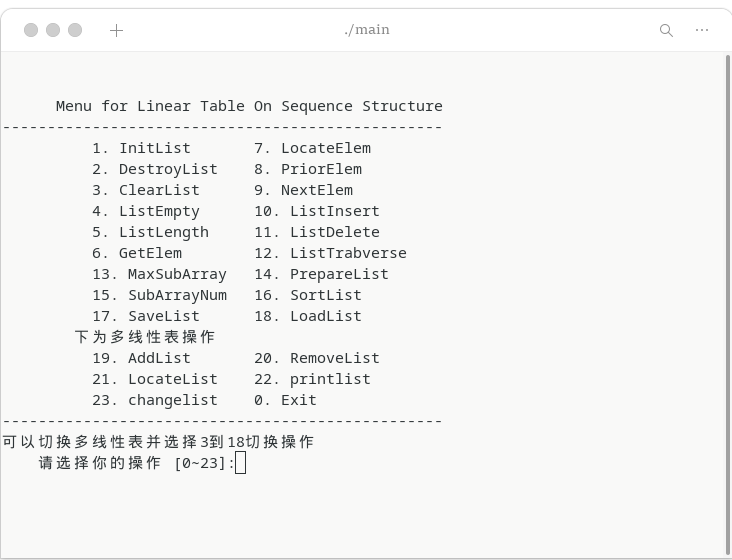
\includegraphics[scale=0.60]{images/1-1.png}
		\caption{系统演示界面}
		\label{fig1-1}
		\end{center}
\end{figure}


\subsection{实验小结}

重点说明在实验中取得的实际经验,例如调试中碰到的典型错误等,不要写套话。画图说明网页的整体框架,进行简要的文字描述等。画图说明网页的整体框架,进行简要的文字描述等。画图说明网页的整体框架,进行简要的文字描述等。画图说明网页的整体框架,进行简要的文字描述等。画图说明网页的整体框架,进行简要的文字描述等。画图说明网页的整体框架,进行简要的文字描述等。画图说明网页的整体框架,进行简要的文字描述等。

\begin{figure}[htb]
	\begin{center}
		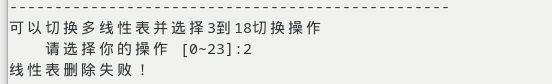
\includegraphics[scale=0.60]{images/1-2.png}
		\caption{在visio里通过文件-打印,把visio图打印成pdf文件}
		\label{fig1-2}
		\end{center}
\end{figure}

画图说明网页的整体框架,进行简要的文字描述等。画图说明网页的整体框架,进行简要的文字描述等。画图说明网页的整体框架,进行简要的文字描述等。画图说明网页的整体框架,进行简要的文字描述等。画图说明网页的整体框架,进行简要的文字描述等。画图说明网页的整体框架,进行简要的文字描述等。画图说明网页的整体框架,进行简要的文字描述等。

\begin{figure}[htb]
	\begin{center}
		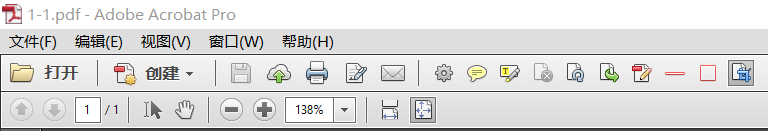
\includegraphics[scale=0.50]{images/1-3.png}
		\caption{用pdf阅览器的工具,对打印得到pdf图做适当的裁剪}
		\label{fig1-3}
	\end{center}
\end{figure}

其实吧,用Latex写公式也不是很难,请参照公式\ref{equ_loss}。画表格就更简单了,请看表\ref{table2}。

\begin{eqnarray}\label{equ_loss}
	\mathcal{L}_{id}=\sum_{j=1}^{c}1\{l_k=j\}\log\frac{\exp(f_j(\textbf{W},x_k))}{\sum\nolimits_{l=1}^{c}\exp(f_l(\textbf{W},x_k))}
\end{eqnarray}

画图说明网页的整体框架,进行简要的文字描述等。画图说明网页的整体框架,进行简要的文字描述等。画图说明网页的整体框架,进行简要的文字描述等。画图说明网页的整体框架,进行简要的文字描述等。画图说明网页的整体框架,进行简要的文字描述等。画图说明网页的整体框架,进行简要的文字描述等。画图说明网页的整体框架,进行简要的文字描述等。

\begin{table}
	\begin{center}
		\setlength{\tabcolsep}{2.0mm}
		\caption{Mean and standard deviation of estimation error (Euler angles) on Pandora. The best performance is in \textbf{bold}.}
		\label{table2}
		\begin{tabular}{c|ccccc}
			\hline
			Method    			        & Data               & Pitch         & Roll           & Yaw              & Accuracy\\
			\hline
			\hline			
			\multirow{5}{*}{POSEidon}   & Depth              & 6.5 $\pm$ 6.6  & 5.4 $\pm$ 5.1  & 10.4 $\pm$ 11.8  & 0.646\\
			& FfD              	 & 6.8 $\pm$ 7.0  & 5.7 $\pm$ 5.7  & 10.5 $\pm$ 14.6  & 0.647\\
			& Gray-level         & 7.1 $\pm$ 6.6  & 5.6 $\pm$ 5.8  & 9.0  $\pm$ 10.9  & 0.639\\
			& Depth + FfD	     & 5.6 $\pm$ 5.0  & 4.9 $\pm$ 5.0  & 9.8  $\pm$ 13.4  & 0.698\\
			& Depth + FfD + MI   & 5.7 $\pm$ 5.6  & 4.9 $\pm$ 5.1  & 9.0  $\pm$ 11.9  & 0.715\\
			\hline
			DRF                         & Depth              & 6.2 $\pm$ 9.5  & 4.6 $\pm$ 6.7  & 9.3  $\pm$ 14.6  & --\\
			\hline
			\multirow{3}{*}{Ours}   	& Depth              & 5.9 $\pm$ 6.2  & 4.5 $\pm$ 4.9  & 8.8  $\pm$ 10.9  & 0.666\\
			& RGB                & 5.5 $\pm$ 5.3  & 4.4 $\pm$ 5.5  & 8.6  $\pm$ 9.3   & 0.698\\
			& RGB + Depth        & 5.0 $\pm$ 4.8  & 4.3 $\pm$ 4.9  & 8.1  $\pm$ 8.3   & \textbf{0.737}\\
			\hline
		\end{tabular}
	\end{center}
\end{table}

\newpage

\section{基于链式存储结构的线性表实现}

描述主页的结构,给出主页截图,描述主要设计思路等,请见图\ref{fig2-1}。描述主页的结构,给出主页截图,描述主要设计思路等。描述主页的结构,给出主页截图,描述主要设计思路等。描述主页的结构,给出主页截图,描述主要设计思路等。描述主页的结构,给出主页截图,描述主要设计思路等。描述主页的结构,给出主页截图,描述主要设计思路等。描述主页的结构,给出主页截图,描述主要设计思路等。

\begin{figure}[htb]
	\begin{center}
		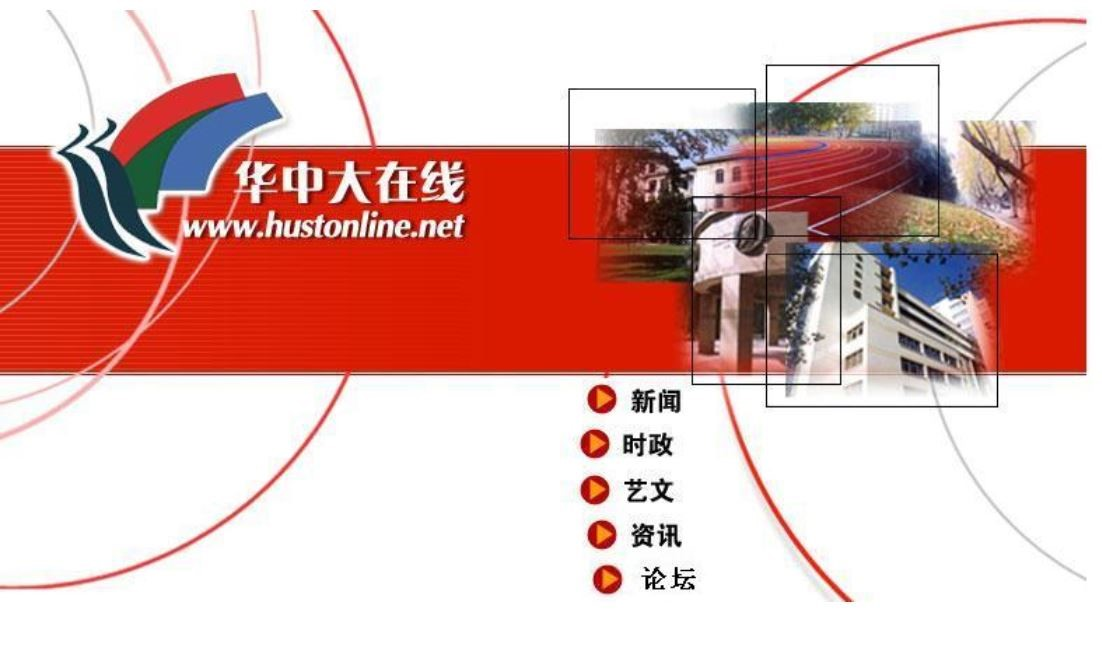
\includegraphics[scale=0.40]{images/2-1.jpg}
		\caption{主页举例}
		\label{fig2-1}
	\end{center}
\end{figure}

\subsection{问题描述}

说明此实验要解决的基本问题。大力出奇迹!!!参考文献无法显示怎么办?陈老师正在想办法解决\cite{STR2021Neurocom, AVS2021Neurocom}!我是参考文献。我是第二小节\cite{Mehrabian1974An}。我是第二小节\cite{Rezaei2014CVPR}。我是第二小节\cite{Ramnath2008IJCV}。

\subsection{系统设计}

包括整体系统结构设计和数据结构设计等。先在文件夹里的bib文件里添加新的参考文献,给每篇参考文献取一个索引的名字,然后再引用比如\cite{STR2021Neurocom}\cite{AVS2021Neurocom, Rezaei2014CVPR}。请注意书籍、期刊论文、专利等bib条目的格式是不一样的。画图说明网页的整体框架,进行简要的文字描述等。画图说明网页的整体框架,进行简要的文字描述等。画图说明网页的整体框架,进行简要的文字描述等。画图说明网页的整体框架,进行简要的文字描述等。画图说明网页的整体框架,进行简要的文字描述等。画图说明网页的整体框架,进行简要的文字描述等。画图说明网页的整体框架,进行简要的文字描述等。

\subsection{系统实现}

主要说明各个主要函数的实现思想,复杂函数可辅助流程图进行说明,函数和系统实现的源代码放在附录中。画图说明网页的整体框架,进行简要的文字描述等。画图说明网页的整体框架,进行简要的文字描述等。画图说明网页的整体框架,进行简要的文字描述等。画图说明网页的整体框架,进行简要的文字描述等。画图说明网页的整体框架,进行简要的文字描述等。画图说明网页的整体框架,进行简要的文字描述等。画图说明网页的整体框架,进行简要的文字描述等。

\subsection{系统测试}

主要说明针对各个函数正常和异常的测试用例及测试结果画图说明网页的整体框架,进行简要的文字描述等。画图说明网页的整体框架,进行简要的文字描述等。画图说明网页的整体框架,进行简要的文字描述等。画图说明网页的整体框架,进行简要的文字描述等。画图说明网页的整体框架,进行简要的文字描述等。画图说明网页的整体框架,进行简要的文字描述等。画图说明网页的整体框架,进行简要的文字描述等。

\begin{figure}[htb] % here top bottom
	\begin{center}
		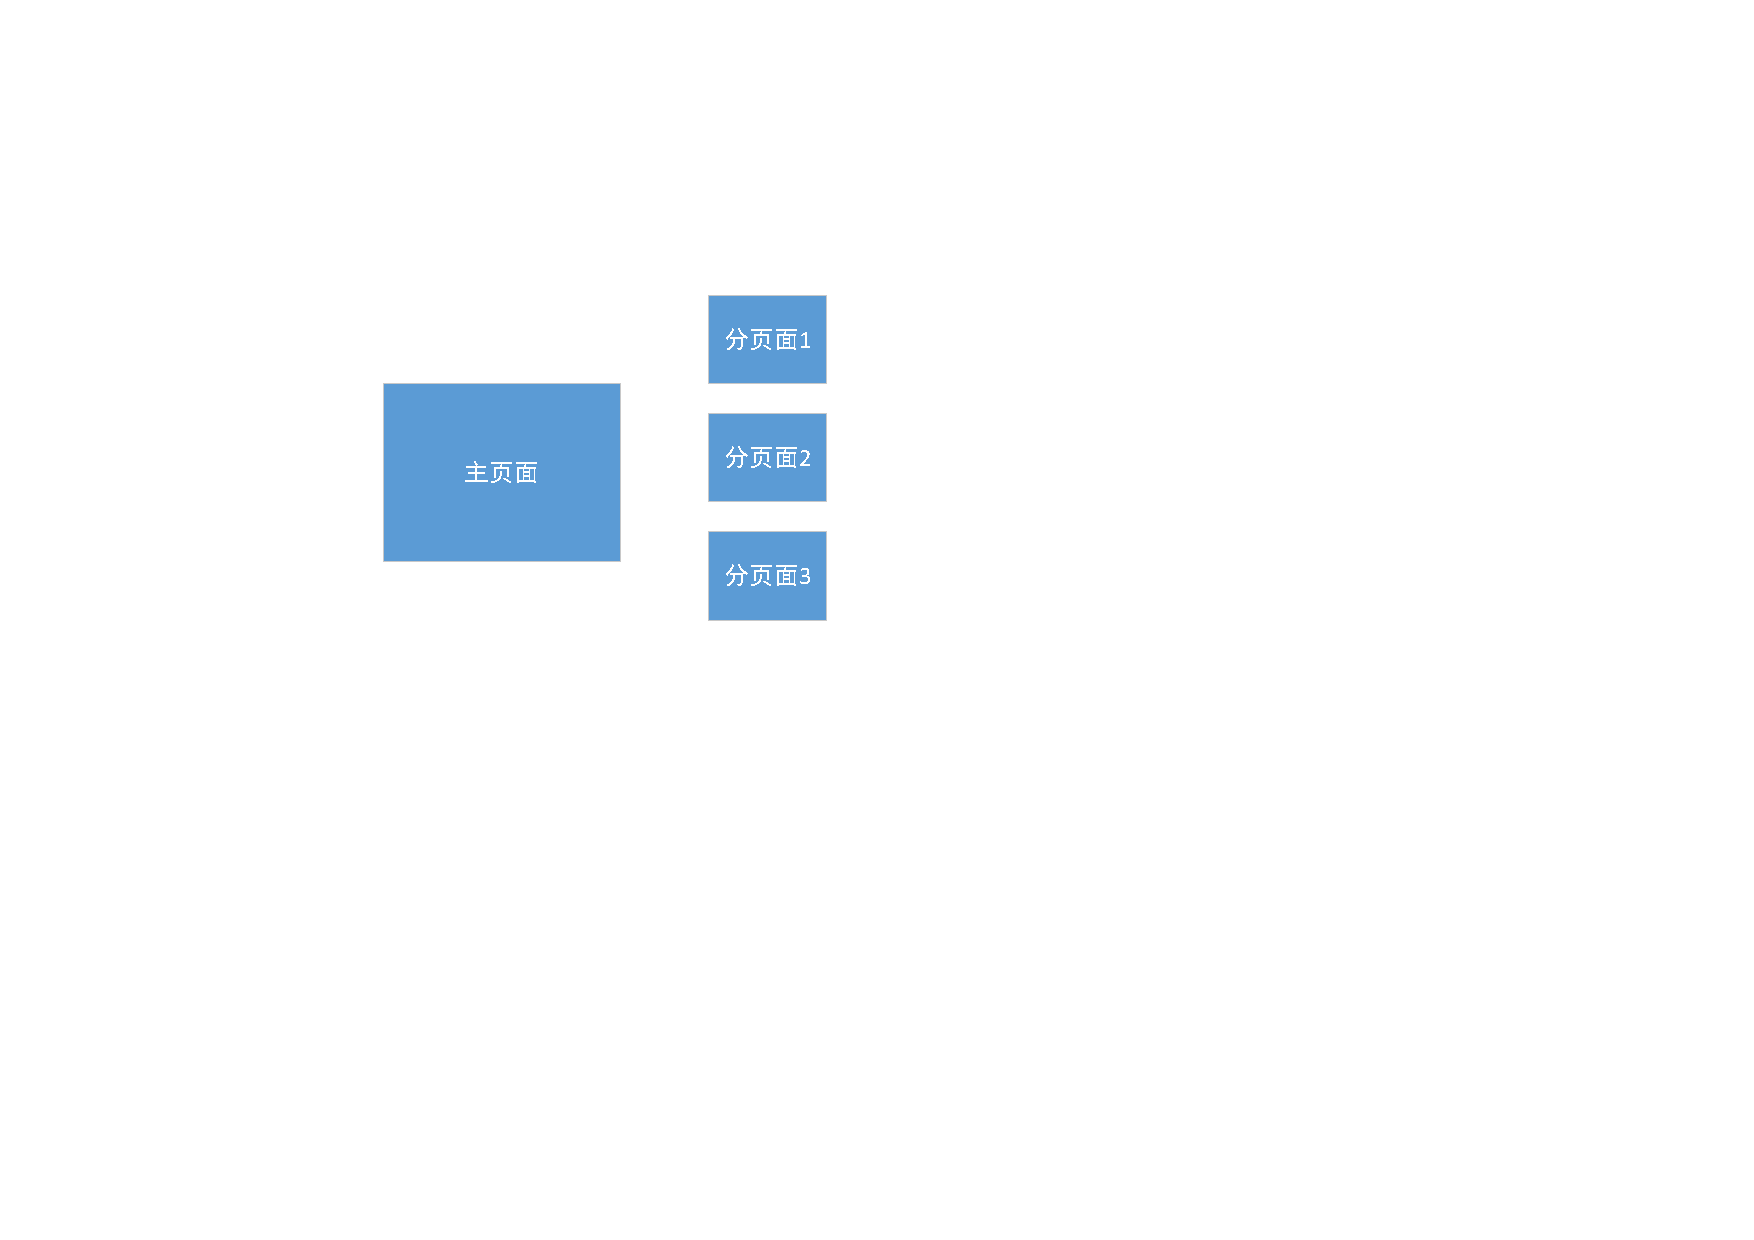
\includegraphics[scale=0.80]{images/1-1.pdf}
		\caption{网页整体框架举例}
		\label{fig4-1}
	\end{center}
\end{figure}

\subsection{实验小结}

\newpage

\section{基于二叉链表的二叉树实现}

给出分页面截图,描述主要设计思路等。给出分页面截图,描述主要设计思路等。给出分页面截图,描述主要设计思路等。给出分页面截图,描述主要设计思路等。

\subsection{问题描述}

说明此实验要解决的基本问题。大力出奇迹!!!参考文献无法显示怎么办?陈老师正在想办法解决\cite{STR2021Neurocom, AVS2021Neurocom}!我是参考文献。我是第二小节\cite{Mehrabian1974An}。我是第二小节\cite{Rezaei2014CVPR}。我是第二小节\cite{Ramnath2008IJCV}。

\subsection{系统设计}

包括整体系统结构设计和数据结构设计等。先在文件夹里的bib文件里添加新的参考文献,给每篇参考文献取一个索引的名字,然后再引用比如\cite{STR2021Neurocom}\cite{AVS2021Neurocom, Rezaei2014CVPR}。请注意书籍、期刊论文、专利等bib条目的格式是不一样的。画图说明网页的整体框架,进行简要的文字描述等。画图说明网页的整体框架,进行简要的文字描述等。画图说明网页的整体框架,进行简要的文字描述等。画图说明网页的整体框架,进行简要的文字描述等。画图说明网页的整体框架,进行简要的文字描述等。画图说明网页的整体框架,进行简要的文字描述等。画图说明网页的整体框架,进行简要的文字描述等。

\subsection{系统实现}

主要说明各个主要函数的实现思想,复杂函数可辅助流程图进行说明,函数和系统实现的源代码放在附录中。画图说明网页的整体框架,进行简要的文字描述等。画图说明网页的整体框架,进行简要的文字描述等。画图说明网页的整体框架,进行简要的文字描述等。画图说明网页的整体框架,进行简要的文字描述等。画图说明网页的整体框架,进行简要的文字描述等。画图说明网页的整体框架,进行简要的文字描述等。画图说明网页的整体框架,进行简要的文字描述等。

\subsection{系统测试}

主要说明针对各个函数正常和异常的测试用例及测试结果画图说明网页的整体框架,进行简要的文字描述等。画图说明网页的整体框架,进行简要的文字描述等。画图说明网页的整体框架,进行简要的文字描述等。画图说明网页的整体框架,进行简要的文字描述等。画图说明网页的整体框架,进行简要的文字描述等。画图说明网页的整体框架,进行简要的文字描述等。画图说明网页的整体框架,进行简要的文字描述等。

\begin{figure}[htb] % here top bottom
	\begin{center}
		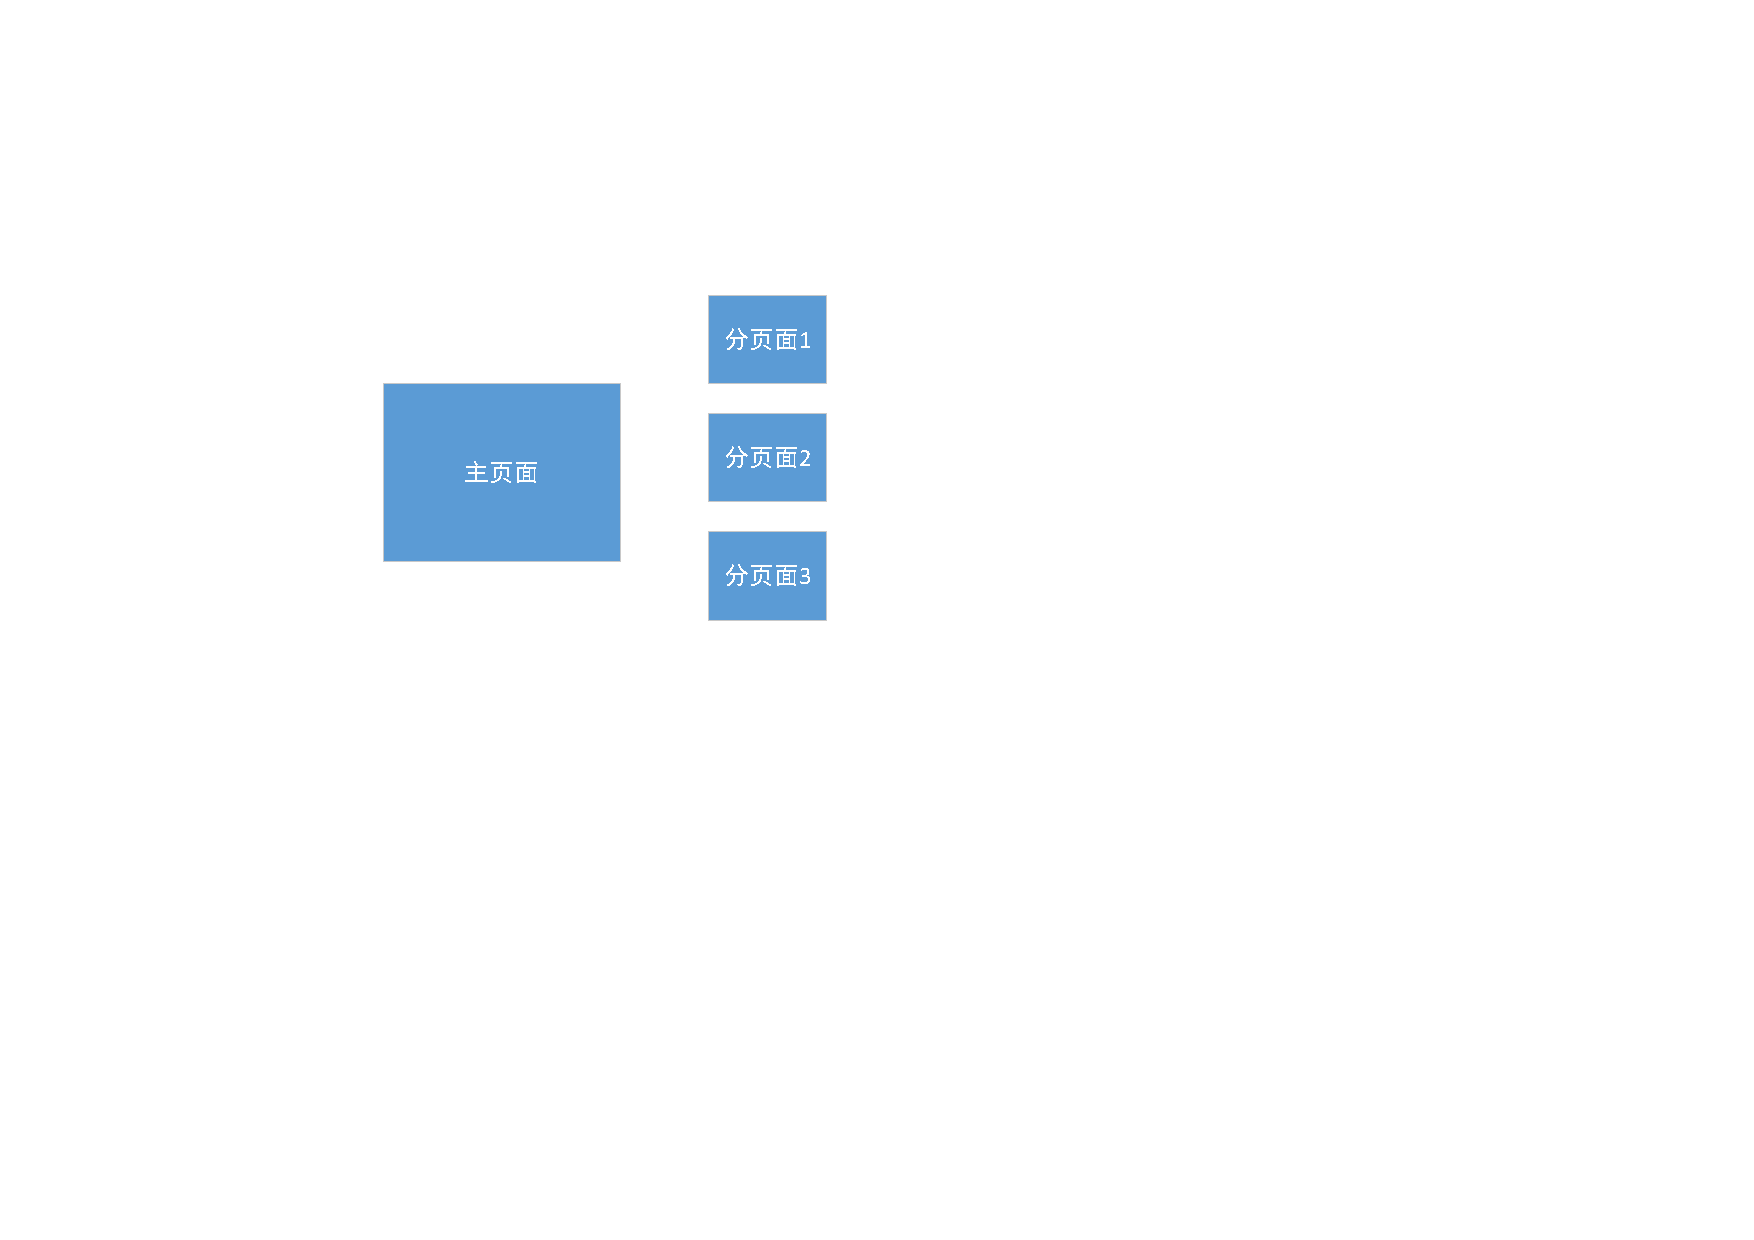
\includegraphics[scale=0.80]{images/1-1.pdf}
		\caption{网页整体框架举例}
		\label{fig3-1}
	\end{center}
\end{figure}

\subsection{实验小结}

如果实验报告中要用到算法伪代码,请参考算法\ref{alg:1},也可以参考算法\ref{alg:2}。如果实验报告中要用到算法伪代码,请参考算法\ref{alg:1},也可以参考算法\ref{alg:2}。如果实验报告中要用到算法伪代码,请参考算法\ref{alg:1},也可以参考算法\ref{alg:2}。如果实验报告中要用到算法伪代码,请参考算法\ref{alg:1},也可以参考算法\ref{alg:2}。

\begin{shaded*}\begin{alg}{一个复杂算法}
		\label{alg:1}
		\begin{algorithmic}
			\Input Two numbers $a$ and $b$
			\Output The sum of $a$ and $b$
			\Procedure{A-Plus-B}{$a, b$}
			\If $a = 0$
			\State \Return $b$
			\EndIf
			\State $res \gets 0$
			\While{$b \neq 0$}
			\State Increase $res$ by $1$
			\State $b \gets b - 1$
			\EndWhile
			\State \Return $res$
			\EndProcedure
		\end{algorithmic}
\end{alg}\end{shaded*}

如果实验报告中要用到算法伪代码,请参考算法\ref{alg:1},也可以参考算法\ref{alg:2}。如果实验报告中要用到算法伪代码,请参考算法\ref{alg:1},也可以参考算法\ref{alg:2}。如果实验报告中要用到算法伪代码,请参考算法\ref{alg:1},也可以参考算法\ref{alg:2}。如果实验报告中要用到算法伪代码,请参考算法\ref{alg:1},也可以参考算法\ref{alg:2}。

\begin{algorithm}[h] 
	\caption{一个更复杂算法}
	\begin{algorithmic}[1]
		\State Initialization: $I_{xy}$, $z_{f}=Zeros(128, 128)$; 
		\For{$0\leq n \textless N$}
		\State $i=\lfloor x_n \rfloor+64$, $j=\lfloor y_n \rfloor + 64$
		\If{$z_n<0$ and $|z_n|>|z_{f}(i,j)|$};
		\State $z_{f}(i,j)=z_n$;
		\EndIf
		\State $I_{xy}(i,j)=z_{f}(i,j)$;
		\EndFor 
	\end{algorithmic}\label{alg:2}
\end{algorithm}

\newpage

\section{基于邻接表的图实现}

\subsection{问题描述}

说明此实验要解决的基本问题。大力出奇迹!!!参考文献无法显示怎么办?陈老师正在想办法解决\cite{STR2021Neurocom, AVS2021Neurocom}!我是参考文献。我是第二小节\cite{Mehrabian1974An}。我是第二小节\cite{Rezaei2014CVPR}。我是第二小节\cite{Ramnath2008IJCV}。

\subsection{系统设计}

包括整体系统结构设计和数据结构设计等。先在文件夹里的bib文件里添加新的参考文献,给每篇参考文献取一个索引的名字,然后再引用比如\cite{STR2021Neurocom}\cite{AVS2021Neurocom, Rezaei2014CVPR}。请注意书籍、期刊论文、专利等bib条目的格式是不一样的。画图说明网页的整体框架,进行简要的文字描述等。画图说明网页的整体框架,进行简要的文字描述等。画图说明网页的整体框架,进行简要的文字描述等。画图说明网页的整体框架,进行简要的文字描述等。画图说明网页的整体框架,进行简要的文字描述等。画图说明网页的整体框架,进行简要的文字描述等。画图说明网页的整体框架,进行简要的文字描述等。

\subsection{系统实现}

主要说明各个主要函数的实现思想,复杂函数可辅助流程图进行说明,函数和系统实现的源代码放在附录中。画图说明网页的整体框架,进行简要的文字描述等。画图说明网页的整体框架,进行简要的文字描述等。画图说明网页的整体框架,进行简要的文字描述等。画图说明网页的整体框架,进行简要的文字描述等。画图说明网页的整体框架,进行简要的文字描述等。画图说明网页的整体框架,进行简要的文字描述等。画图说明网页的整体框架,进行简要的文字描述等。

\subsection{系统测试}

主要说明针对各个函数正常和异常的测试用例及测试结果画图说明网页的整体框架,进行简要的文字描述等。画图说明网页的整体框架,进行简要的文字描述等。画图说明网页的整体框架,进行简要的文字描述等。画图说明网页的整体框架,进行简要的文字描述等。画图说明网页的整体框架,进行简要的文字描述等。画图说明网页的整体框架,进行简要的文字描述等。画图说明网页的整体框架,进行简要的文字描述等。

\begin{figure}[htb] % here top bottom
	\begin{center}
		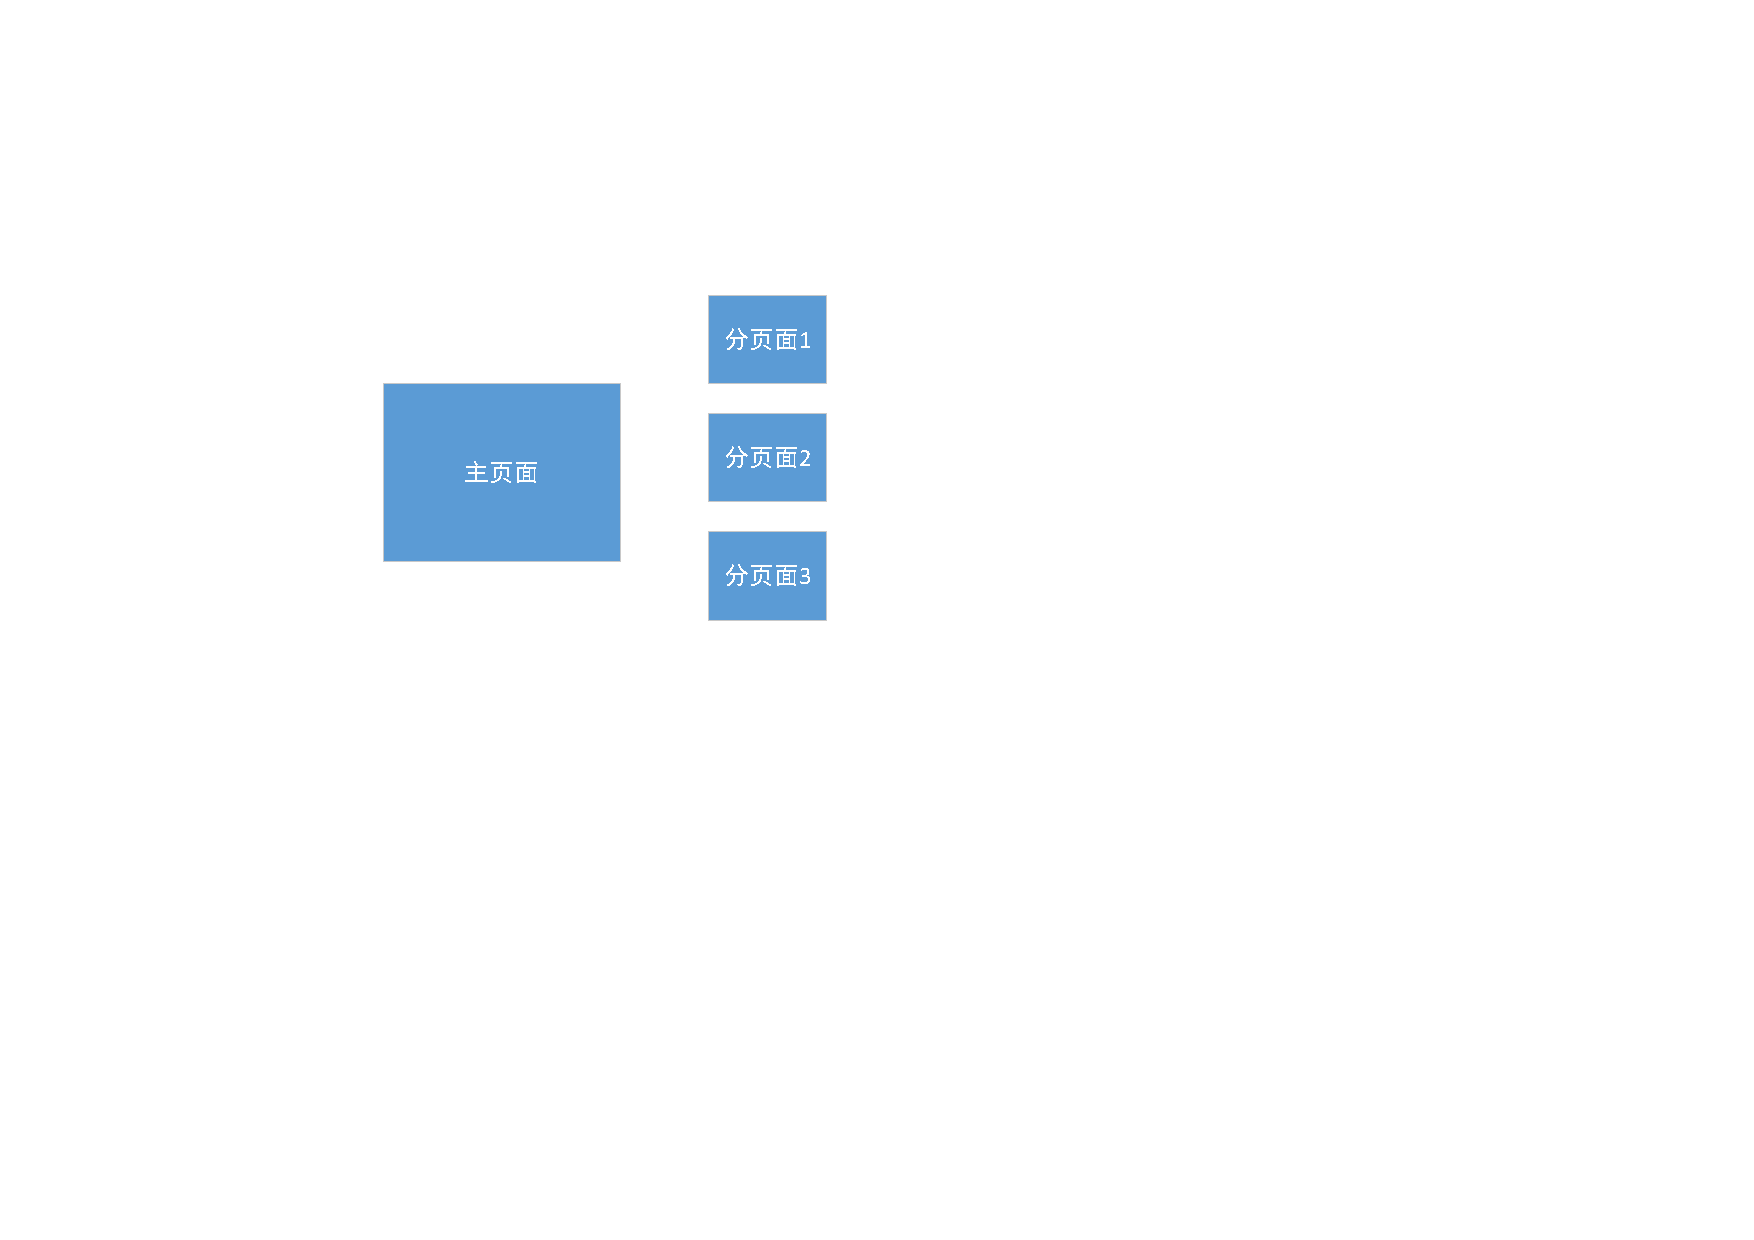
\includegraphics[scale=0.80]{images/1-1.pdf}
		\caption{网页整体框架举例}
		\label{fig5-1}
	\end{center}
\end{figure}

\subsection{实验小结}

\newpage

\section{课程的收获和建议}

描述通过学习该专题,有何收获,有何建议,如某专题可适当减少讲授时间、某专题可适当增加讲授内容和时间等。描述通过学习该专题,有何收获,有何建议,如某专题可适当减少讲授时间、某专题可适当增加讲授内容和时间等。描述通过学习该专题,有何收获,有何建议,如某专题可适当减少讲授时间、某专题可适当增加讲授内容和时间等。描述通过学习该专题,有何收获,有何建议,如某专题可适当减少讲授时间、某专题可适当增加讲授内容和时间等。

\subsection{基于顺序存储结构的线性表实现}

描述通过学习计算机基础知识专题,有何收获,有何建议,如某专题可适当减少讲授时间、某专题可适当增加讲授内容和时间等。描述网页的设计和实现过程中遇到的问题及如何解决。描述网页的设计和实现过程中遇到的问题及如何解决。描述网页的设计和实现过程中遇到的问题及如何解决。描述网页的设计和实现过程中遇到的问题及如何解决。描述网页的设计和实现过程中遇到的问题及如何解决。描述网页的设计和实现过程中遇到的问题及如何解决。描述网页的设计和实现过程中遇到的问题及如何解决。描述网页的设计和实现过程中遇到的问题及如何解决。

\subsection{基于链式存储结构的线性表实现}

描述通过学习文档撰写工具LaTeX专题,有何收获,有何建议,如某专题可适当减少讲授时间、某专题可适当增加讲授内容和时间等。描述通过学习文档撰写工具LaTeX专题,有何收获,有何建议,如某专题可适当减少讲授时间、某专题可适当增加讲授内容和时间等。

\subsection{基于二叉链表的二叉树实现}

描述通过学习编程工具Python专题,有何收获,有何建议,如某专题可适当减少讲授时间、某专题可适当增加讲授内容和时间等。描述通过学习编程工具Python专题,有何收获,有何建议,如某专题可适当减少讲授时间、某专题可适当增加讲授内容和时间等。

\subsection{基于二叉链表的二叉树实现}

描述通过学习计算机基础知识专题,有何收获,有何建议,如某专题可适当减少讲授时间、某专题可适当增加讲授内容和时间等。描述通过学习计算机基础知识专题,有何收获,有何建议,如某专题可适当减少讲授时间、某专题可适当增加讲授内容和时间等。


\nocite{*} %% 作用是不对文献进行引用,但可以生成文献列表

\bibliographystyle{Experimental_Report}
\bibliography{Experimental_Report}
\setcounter{secnumdepth}{0}
\appendix

\section{附录A 基于顺序存储结构线性表实现的源程序}

\noindent
/* Linear Table On Sequence Structure */\\
\#include <stdio.h>\\
\#include <malloc.h>\\
\#include <stdlib.h>\\

\noindent
/*---------page 10 on textbook ---------*/\\
\#define TRUE 1\\
\#define FALSE 0\\
\#define OK 1\\
\#define ERROR 0\\
\#define INFEASTABLE -1\\
\#define OVERFLOW -2\\
\newpage
\section{附录B 基于链式存储结构线性表实现的源程序}
\newpage
\section{附录C 基于二叉链表二叉树实现的源程序}
\newpage
\section{附录D 基于邻接表图实现的源程序}

\end{document}